\subsection{Astrobiology System Design}
\label{sec:Astrobiology Design}
%Fre'Etta, I think we need to mention the design change to the pump and clean box, since it was a big change that affected our mission objectives


The collection assembly was initially designed as a four-compartment structure, with two collection and two control containers, two pumps, two pump heaters, and two solenoids. Due to weight and current draw  limitations, the assembly was redesigned as a two-compartment structure, with one collection and one control container,  one pump, one heater and two solenoids. The clean box and containers were machined from impact-resistant UHMWPE~\cite{cleanbox}. The control container was connected to a solenoid that remained closed until post-sanitation procedures were performed. The sample collection container was connected to a vacuum pump located outside of the clean box structure. The heater was attached to the pump to prevent a cold start. Once float altitude was reached, the solenoid connected to the sample collection container was opened and the pump was powered on; allowing air to flow to the collection container. Each container held \SIrange{30}{40}{\milli\liter} of a \SI{15}{\%} sterile glycerol solution. A 316 Stainless Steel \SI{1/4}{\inch} NPT Vent to Atmosphere Vitron Seal Valve was embedded in each of the compartments, to accommodate for the pressure changes that occurred with the variations in altitude over the course of the flight~\cite{valve}, as well as operate as the sample exhaust.  The left side of Figure~\ref{fig:pump} displays the clean box structure, showing the bottles inside and the lids with the openings for the sample and exhaust tubing, while the right side of Figure~\ref{fig:pump} shows the 3D rendering of the sampling pump. 


\begin{figure}[!h] 
\begin{center}
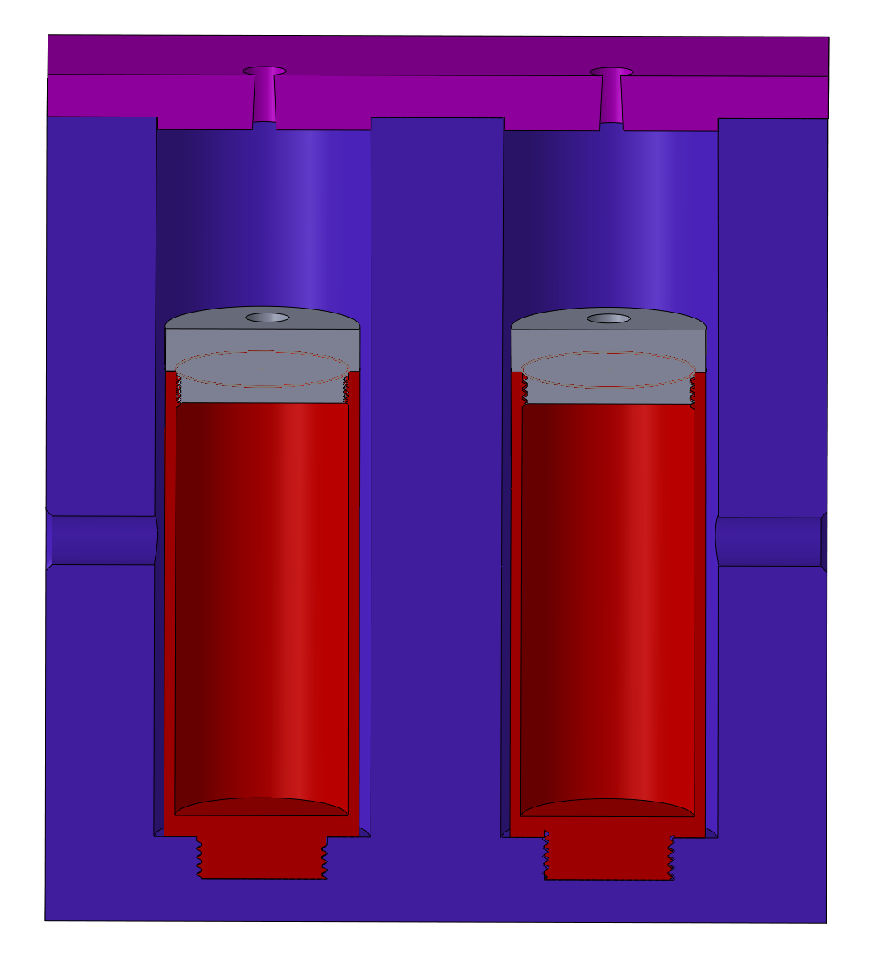
\includegraphics[scale=.3]{./Figures/CB.PDF}
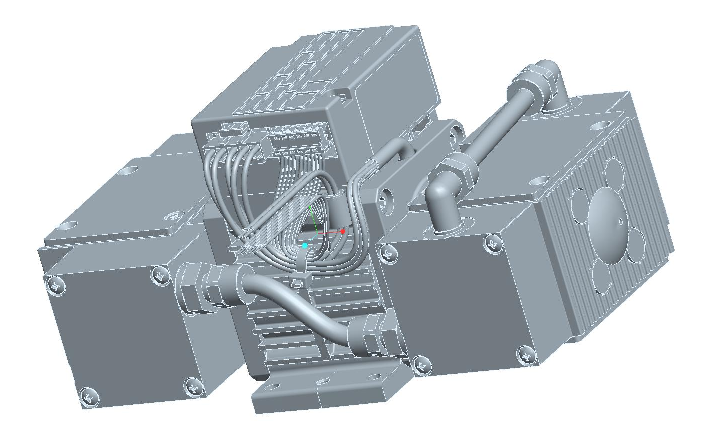
\includegraphics[scale=.7]{./Figures/Pump.pdf}
\caption{{\bf Left:} Cross-section view of the clean box with experimental and control containers. {\bf Right:} KNF N84-4 commercial gas-sampling diaphragm vacuum pump.}
\label{fig:pump}
\end{center}
\end{figure} 
